\documentclass[11pt]{book}
%Gummi|063|=)
\title{\textbf{Complete this book }}
\author{Deebul Nair}
\date{}

\usepackage{amsmath}
\usepackage{todonotes}
\begin{document}

\maketitle


\chapter{Introduction}


In this thesis, we consider methods for learning dynamical models for time series with complex and uncertain behavior patterns. Specifically, we address how Bayesian nonparametric methods can be used to provide a flexible and computationally efficient structure for learning and inference of these complex systems.
\section{ The Right Kind of Smarts }
Smart robots humbly predict our needs and modestly adjust as little as possible to accommodate them. Imagine if your robot could learn how you arrange the breakfast table by looking at the data from previous days? 
We can also have a conversation with smart robots. They can tell us what they’re up to when we ask, or tell us something’s wrong when it’s essential. They can observe our lives and provide small insights we don’t even notice. They can pass along helpful information to humans, like observing our sleep habits and tell us when we are not having adequate sleeps.
We can have a new relationship with our robots, one where the previously mute boxes of plastic and metal become new platforms—not as replacement, but for meaning and value. By learning how we interact with our homes and how we live our lives, robots will be able to provide services to us we can’t see right now. They’ll set themselves up and fit into the existing household by knowing what—and who—is there and adapting to them. Robots will grow and change with you and the house.

robots with a greater awareness of the world around them.
\chapter{Basics}

IN this background chapter, we review the statistical methodologies 
The goal of this chapter is to provide the basic information regarding Bayesian methods of machine learning used in the thesis. A good introduction to the field can be found in books of Bishop \cite{}, Kirchop \cite{} and LeeWagenmakers \cite{} . 

\section{Bayesian Model Learning}

Bayesian models are represented as probability distributions. Probability is used to quantify "uncertainty" or "Degree of belief". The models are initialized with some prior probabilities(beliefs). The observed data are used to update the prior beliefs to become posterior beliefs.

We can explain this with an example. Assume we have a bag with 50 marbles with 2 colours, red and blue. We randomly take 10 marbles out of the bag and observe their colour with replacement. What we have to model is, our belief of the numbers of colours inside the bag, in bayesian  terms colour distribution in the bag, which we can define as $\theta$ . We cannot directly observe the bag. All that we can observe are the colours of the 10 picked marbles.

Before we do anything else we need to specify our prior belief with respect to the colour distribution $\theta$ . This belief needs to be expressed as a probability distribution, called the \emph{prior distribution}. A reasonable "prior distribution" denoted by $p(\theta)$ is one which takes uniform value between 0 and 1. Lets assume $p(\theta)$ is belief of red marbles in bag then $1 - p(\theta)$  is the belief of blue marbles in the bag. This uniform distribution is shown as dotted line in the figure 

Now we consider the observed colour of the 10 marbles from the bag. We observe 8 red marbles and 2 blue marbles. After observing the data, the updated knowledge about $\theta$ is described by a \emph{posterior distribution}, denoted by $p(\theta | D)$, where D indicates the observed data. The distribution represents the updated belief after observing the colour picked marbles. Bayes rule specifies how we can combine the information from the data, that is how to determine the posterior distribution $p (\theta | D)$ using  the prior distribution $p(\theta)$ and the likelihood  $p (D | \theta)$ :
\begin{equation}
	p(\theta | D) = \frac{p(D | \theta) p(\theta)}{p(D)}
\end{equation}

The equation is often verbalized as :
\begin{equation}
	posterior = \frac{likelihood * prior}{marginal likelihood}
\end{equation}

We note here that the posterior distribution is a combination of the prior information we had and what we have learned from the data. 



\missingfigure{Image of the prior posterior}

\section{Prediction}

\section{Distributions }

Dirichlet, Categorical, Bernoulli 

Conjugate prior  need to explain this 

\section{Graphical Models}

\section{Probabilistic Programming}

Until recently, Bayesian Model learning have been limited in scope, and have been hard to apply to many real-world applications. Probabilistic programming is a new approach which makes Bayesian learning easier to build and more applicable. 
\subsection{PyMC3}

\subsection{BayesPy}

\subsection{WebPPL}

\section{Model Evaluation}

\section{DIKW Pyramid }

%######################################################################

%\chapter{Modelling User Location Preferences }
\label{chapter:Human location}
Domestic service robots in future should be able to gather knowledge about all the locations in the home, the user likes to hang around. Additionally they should also know the time period when the users occupy their favourite places. This acquired knowledge of the users location preference shall enable the robots to make informed decisions while assisting the user. For example what time to clean a particular room based on least unoccupied time period or when to turn on the heater of the room. 

In this chapter we focus on this knowledge accession of users location preference based on spatio-temporal observations made by the robot. The advancement in long term autonomous navigation \cite{krajnik_life-long_2015} and the rapid adoption of databases in the robots \cite{niemueller2012generic}, has made the information collection for such knowledge generation possible in service robots. However even with these advancements there are some challenges which still needs to be addressed.  In more details, these challenges are the  (i) modelling users location preference  (ii) prediction of users future locations  (iii) learning all these with sporadic observations made by the robots. 

Significant progress has been made the problem by researchers in the field of human location behaviour, which is to learn the patterns in human location outdoors. Approaches for learning routine mobility  range from purely temporal  (\cite{mcinerney2013modelling, scellato2011nextplace}), spatial  (\cite{gao2012exploring,song2006evaluating}), to a combination  of  both   (\cite{eagle2009eigenbehaviors}). Non-parametric Bayesian methods are also gaining popularity given their ability to refine models as more data arrives. Chen et al.  (2012) used a Gaussian process to model congestion on road networks, while Gao et al.  (2012) used a hierarchical Pitman Yor process to model check-in behaviour on location-based social networks. Indoor human location behaviour was studied by \cite{krajnik_wheres_2015} using Fourier transform methods and Gaussian mixture models. 

While \cite{krajnik_wheres_2015}  work is first step towards learning human mobility behaviour in indoor environments, it failed to address the challenge of sparse dataset in domestic robots. As we have discussed earlier the observations on which the knowledge has to be learned, are sparse. We aim to demonstrate in this chapter that, by using Bayesian models, we can capture the human behaviour patterns in a sparse dataset.

We build Bayesian models which incorporate explicit domain knowledge and the structural knowledge about our data. Human behaviours are periodic in nature with a daily cycle. The models developed use this domain knowledge to extract the patterns emerging from the data caused by periodicity.


\section{Dirichlet Categorical Model }

Dirichlet Categorical (DC) model  is a two-level Bayesian model. The basic idea is that observations of each time period is characterized by a distribution over the possible locations.

In chapter \ref{chapter: object} and \ref{chapter:occupancy} we learned the pattern in the user preference in a single location. For modelling single location based on the presence and absence data we used the Bernoulli distribution to quantify the preference. Here we would like to model the user preference over multiple location in a single model. For modelling more than 2 discrete outcomes, we can use Multinomial or Categorical distribution. In our model we have selected Categorical distribution as the input data to our problem comes sequentially. 

The data are the observed human location $x_{ij}$ for $i = 1 \dots T$ time periods and then $j = 1, \dots , N$  are the observations.  We assume that the latent pattern in the persons location per period are distributed as a categorical distribution. The number of periods $T$ for our model is fixed to 24 corresponding to the number of hours in a day. 

The Dirichlet-Categorical model is the generalization of the Beta-Binomial model to multiple classes of a categorical or multinomial distribution. The conjugate prior for the categorical distribution is the Dirichlet distribution. The model estimates the posterior distribution of $\theta_i$ given our current data and prior beliefs. Our prior beliefs are encoded in the model through the hyper-parameter $\alpha$, which represents pseudo-counts of what we believe the data should look like – typically set as 1's for weak uniform beliefs. The probabilistic graphical model of  DCM is shown in Figure~\ref{dcm}

\noindent
\begin{figure}[htp]

\begin{minipage}{0.3\textwidth}
\centering

\tikz {
\node [const]                   (alpha) {$\alpha$};
\node [below=of alpha, latent]   (theta) {$\theta_i$};
\node [below=of theta, obs]      (x)     {$x_{ij}$};
\edge {alpha} {theta};
\edge {theta} {x};
\plate {trials} { (x)} {j location};
\plate {bags} { (theta) (x) (trials)} {i time};
}

\end{minipage}%
\begin{minipage}{0.7\textwidth}

\begin{equation*}
	\alpha = <1, 1, .... , 1 > 
\end{equation*}
\begin{equation*}
	\theta_i  \sim Dirichlet (\alpha)
\end{equation*}
\begin{equation*}
	x_{ij} \sim Categorical (\theta_i)
\end{equation*}
\end{minipage}
\caption[Dirichlet categorical graphical model representation]{Graphical model representation of DCM. The boxes are ``plates" representing replicates. The outer plates represents hours of a day, while the inner plate represents the choice of locations within each hour.}
\label{dcm}
\end{figure}

With the graphical model, the dependencies among the many variables can be captured concisely. The boxes are ``plates” representing replicates. The outer plate represents the hours of the day, while the inner plate represents the repeated choice of locations within each hour. Thus:

	$\alpha$ is  parameter of the dirichlet prior on per-period location distribution, 
	
	$\theta_i$ is the location distribution for period $i$  ,
	
	$x_{ij}$ is the observed location of the person in period $i$.
	
The $ x_{ij}$ are the only observable variables, and the other variables are latent variables. 

\section{Hierarchical Dirichlet Categorical Model}
\label{sec: HDCM}

Observations made only by a domestic robot using internal sensors and not using any external sensors creates the serious problem of sparsity. There are very much likely that some time periods there will be no observations available to learn. Maximum likelihood estimates of the categorical parameters assign uniform probability to the locations in these time periods. The standard approach to cope with this problem is to sharing statistical strength between time periods: it is as if the location we observe for each time period also provides weaker indirect location relevant to other time periods. In machine learning and statistical science this phenomenon is often called \emph{learning to learn} or \emph{transfer learning}. Intuitively, knowing something about the location of person in the 9'o clock can help in gaining some information at 10'o clock. 

By placing a Dirichlet hyper-prior on the several Dirichlet parameter we obtain the  Hierarchical Dirichlet Categorical  (HDC) model. The hyper-prior makes it possible for sharing the learned knowledge from one prior to another. Thus learning about the location pattern at a higher level of abstraction helps to share it with the lower levels which have no observations.

The probabilistic graphical model of  hierarchical model is shown in Figure \cite{hdcm}

\noindent
\begin{figure}[htp]

\begin{minipage}{0.3\textwidth}
\centering

\tikz {
\node [const]                    (alpha) {$\alpha$};
\node [below=of alpha, latent]   (beta)  {$\beta$};
\node [below=of beta, latent]    (theta) {$\theta_i$};
\node [below=of theta, obs]      (x)     {$x_{ij}$};
\edge {alpha} {beta};
\edge {beta} {theta};
\edge {theta} {x};
\plate {trials} { (x)} {j location};
\plate {bags} { (theta) (x) (trials)} {i time};
}

\end{minipage}%
\begin{minipage}{0.7\textwidth}

\begin{equation*}
	\alpha = <1, 1, .... , 1 > 
\end{equation*}
\begin{equation*}
	\beta \sim Dirichlet (\alpha)
\end{equation*}
\begin{equation*}
	\theta_i  \sim Dirichlet (\beta)
\end{equation*}
\begin{equation*}
	x_{ij} \sim Categorical (\theta_i)
\end{equation*}
\end{minipage}
\caption[Hierarchical dirichlet categorical graphical model representation]{Hierarchical Dirichlet Categorical Model. The boxes are ``plates" representing replicates. The outer plates represents hours of a day, while the inner plate represents the choice of locations within each hour.}
\label{hdcm}
\end{figure}

The model can be explained as:

	\boldmath{$\alpha$} is  constant dirichlet prior for the hyperprior, 
	
	$\beta$ is a Dirichlet hyperprior,
	
	$\theta_i$ is the location distribution for period $i$  ,
	
	$x_{ij}$ is the observed location of the person in period $i$.
	
Thus we have categorical variables dependent on multiple priors sharing a hyperprior.


\section{Experiments}

We give an empirical performance analysis of the above models to determine their capabilities of learning user behaviour and preferences. We first conducted experiments on synthetic dataset to verify if the evaluate the proposed models can learn and the number of observations required for making accurate predictions. Then we compare the DC and HDC models on their capabilities to learn when there is absence of data. Finally we evaluate the models predicting capabilities on a real dataset collected about human location in a home.

The goal of the experiments are to verify 
\begin{itemize}
	\item the robot is able to learn users location preferences.
	\item performance of HDC model compared to DC model.
	\item performance of HDC model with standard machine learning algorithms
	\item search time to locate a person.
\end{itemize}


\section{Model Learning Validation}

Before we start learning on the real dataset we want to validate the proposed models using synthetic dataset. The synthetic dataset consist of observations made by a robot generated using known ground truth probabilities. The models learn using the synthetic dataset and generate the learned probabilities. The distance between the learned probability and ground truth probability is used to quantify the learning of the model. 

\subsection{Simulated Dataset: Kitchen Object Dataset}

To demonstrate the learning in the proposed approach we have generated a kitchen object dataset. The dataset consist of simulated observations of a cup in a kitchen environment made by a domestic robot \cite{fig:eval_cup}. The robot can scan 4 locations in the kitchen: sink, counter-top, stove and cabinet. The time of the scan is discretized into 3 times of the day: morning, afternoon and night. 

The generative process for each possible observation in the dataset 
\begin{itemize}
    \item Choose $ \theta \sim Dirichlet (\alpha)$  (Distribution of object over location-time)
    \item Choose randomly the time period $i$.
	\item Choose the location $x_n$ $\sim$ Categorical$ (\theta_i)$ , where the object was observed.
	\end{itemize}

Ground truth of the distribution in the object location distribution over time in shown in Figure \ref{absent-gt}. The figure represents the hinton plot of the underlying Dirichlet distributions. Hinton plot are a way of visualizing probabilities. The size of the white square in the plot quantifies the belief of the probability. Higher the size of the box higher the probability. Thus for probability 1 we have a complete white box and gray means 0 probability. In the ground truth probability in Figure \ref{fig:eval_gt} the each row represents the distribution of the object cup at the particular time period. We see a big white box at location:sink and time:night on the bottom left of the plot, while all other boxes for row night are comparatively small. This signifies that the box is more likely to be found in the cabinet in the night than the other places.  We evaluate our models on these synthetic observations.

\begin{figure}
    \centering
    \begin{subfigure}[b]{0.4\textwidth}
        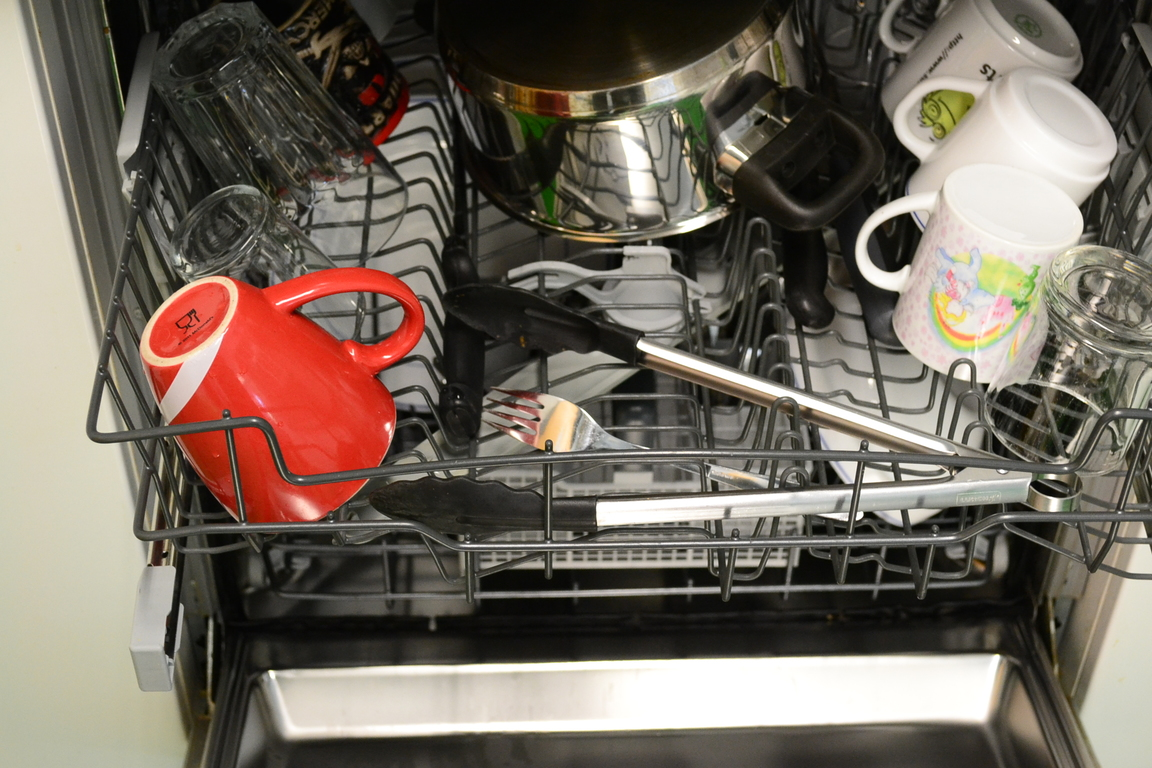
\includegraphics[width=\textwidth]{images/cup_dishwasher.jpg}
        \caption{}
        \label{fig:eval_cup}
    \end{subfigure}
    ~ %add desired spacing between images, e. g. ~, \quad, \qquad, \hfill etc. 
      % (or a blank line to force the subfigure onto a new line)
    \begin{subfigure}[b]{0.5\textwidth}
        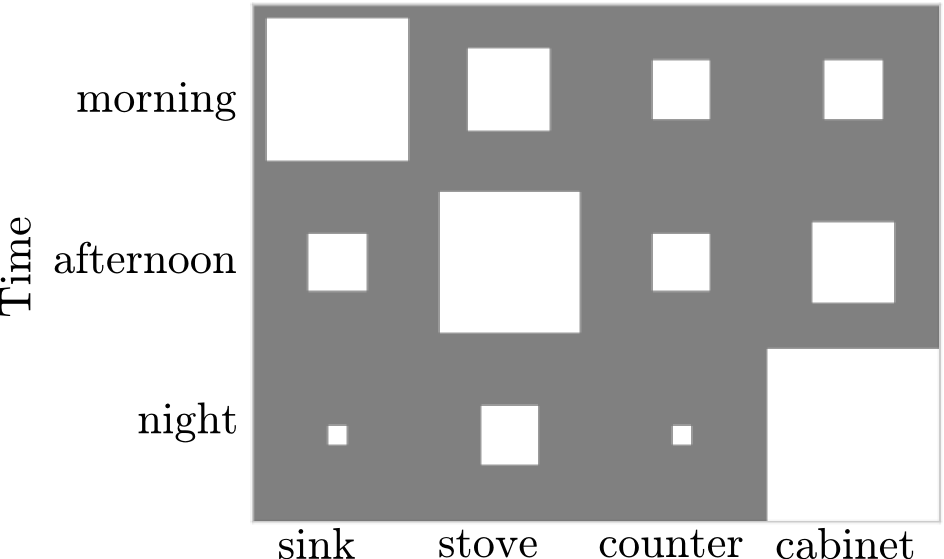
\includegraphics[width=\textwidth]{images/eval_ground_truth.png}
        \caption{}
        \label{fig:eval_gt}
    \end{subfigure}
    \caption[Model Validation dataset generation]{Simulated dataset generation of the cup in different location at different times of the day. Simulated cup locations ground truth probability distribution.
The x-axis represents the locations the y axis represents the timezones. The size of the white box indicates the probability of the object presence.}
\label{}
\end{figure}




\subsection{Posterior Probability Check}
The first method was to visually compare the learned probabilities with the ground truth.  Figure~\ref{fig:eval_gt} we can visually analyse the difference between the learned models of both DC model and HDC model. The leftmost plot \ref{fig:eval_gt} as explained above is the ground truth probabilities from which the observations were generated. We generated a dataset with \textbf{100} observations. The models use the observations and creates its posterior distribution. The middle plot \ref{fig:eval-dc} is the learned posterior probabilities using the DC model while the last plot \ref{fig:eval-hdc} is the posterior probabilities using the DC model presented in this chapter. 

Visually we can observe from the plots both the posterior probabilities of both the models are similar to the ground truth probabilities. Thus we can conclude that the proposed models are converging to the true probabilities. In the next section we quantitatively compare the models using different data size.

\begin{figure}
    \centering
    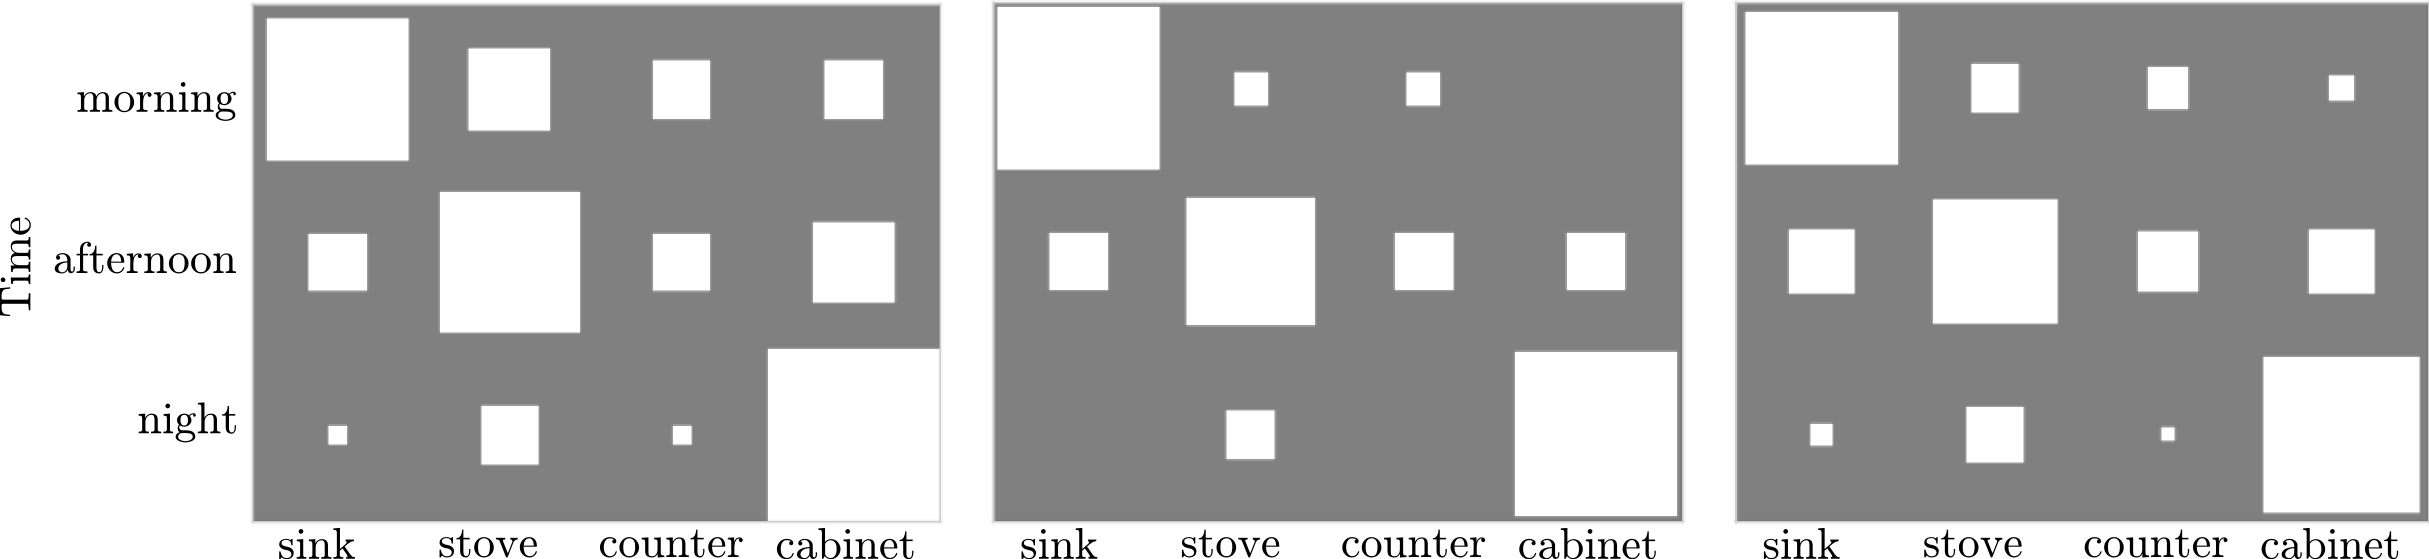
\includegraphics[width=\textwidth]{images/eval_gt_DC_HDC.png}
       
    \begin{minipage}[t]{.35\textwidth}
    %\centering
    \subcaption{Ground Truth}\label{fig:eval_gt_2}
    \end{minipage}%
    \begin{minipage}[t]{.3\textwidth}
    %\centering
    \subcaption{DC model}\label{fig:eval-dc}
    \end{minipage}
    \begin{minipage}[t]{.25\textwidth}
    %\centering
    \subcaption{HDC model}\label{fig:eval-hdc}
    \end{minipage}

\caption[Posterior probabilities of DC and HDC ]{Posterior probabilities of the models : \ref{fig:eval_gt_2} is ground truth of the distribution. \ref{fig:eval-dc} is the learned distribution using the DC model. \ref{fig:eval-hdc} is the learned distribution using the HDC  model . The x-axis represents the locations the y axis represents the timezones. The size of the white box indicates the probability of the object presence }\label{fig:eval-dc-hdc}
    
\end{figure}

\section{Model Comparison}

The goal of the experiments is to empirically validate both Dirichlet-Categorical and Hierarchical-Dirichlet-Categorical model 
learning using different data size. We also validate that HDC can compensate  for lack of observations in some time period by sharing information.

We employ two methods for evaluating the performance of the developed models on the synthetic dataset. We use the adopted Bhattacharyya distance \cite{bhattacharyya1946measure} and Kullback–Leibler divergence \cite{kullback1951information}  (KL Divergence)to quantify the distance between the simulated and the learned Dirichlet distribution.   

\subsection{Bhattacharyya Distance}
Bhattacharyya distance measures the similarity of two discrete or continuous probability distributions. The distance ranges from 0 to $\inf$ with \textbf{0} meaning both probabilities are identical. The  adopted Bhattacharyya distance \cite{rauber2008bhattacharyya} for comparing dirichlet distributions is given by :
\begin{multline}
	D_B (Dir_a (x_1, \dots ,x+n), Dir (y_1, \dots , y_n)) = \nonumber\\
	 \Gamma \Bigg ( \frac{1}{2}  \sum_{i \in {1, \dots, n}} x_i +  \frac{1}{2}\sum_{i \in {1, \dots, n}} y_i\Bigg) + 
	\frac{1}{2}  \sum_{i \in {1, \dots, n}} \Gamma  (x_i) + 
	\frac{1}{2}  \sum_{i \in {1, \dots, n}} \Gamma  (y_i) - \\ 
	\sum_{i \in {1, \dots, n}} \Gamma \bigg (\frac{1}{2}  (x_i + y_i) \bigg) - \frac{1}{2}  \Gamma \Bigg (  \sum_{i \in {1, \dots, n}} x_i \Bigg) + \frac{1}{2}  \Gamma \Bigg ( \sum_{i \in {1, \dots, n}} y_i\Bigg)
\end{multline}

\subsection{Kullback–Leibler Divergence}
Similarly KL divergence also measures the similarity of two discrete or continuous probability distributions. Even for KL divergence, 0 signifies both probabilities are identical.  
The KL divergence between two distributions $p$ and $q$ is given by
\begin{equation*}
	KL (p||q) = \int p (x) \log \frac{p (x)}{q (x)} dx = \left < \log \frac{p (x)}{q (x)}  \right>_{p (x)}
\end{equation*}

Lets suppose we have two Dirichlet distributions $p$ and $q$ with parameters $\alpha$ and $\beta$ respectively, then the KL divergence between Dirichlet distributions\cite{kurt2013} is given by
\begin{equation*}
	\begin{split} 
 KL (p||q) &= \log \Gamma (\alpha_0) - \sum_{k=1}^K \log \Gamma (\alpha_k)   
 - \log \Gamma (\beta_0) \\ &+ \sum_{k=1}^K \log \Gamma (\beta_k)  + \sum_{k=1}^K  (\alpha_k – \beta_k)  (\psi (\alpha_k)-\psi (\alpha_0)) 
\end{split}
\end{equation*}


The only difference being that KL divergence is unsymmetrical while Bhattacharyya distance is symmetric. 

\subsection{Results}
We generated dataset with increasing number of observations from 20 to 800. For each observation set we trained both the models and their corresponding distance with the ground truth were recorded. The process was repeated 100 times for each sample set.

\begin{figure}[htp]
\centering

\begin{subfigure}{.45\textwidth}
  \centering
  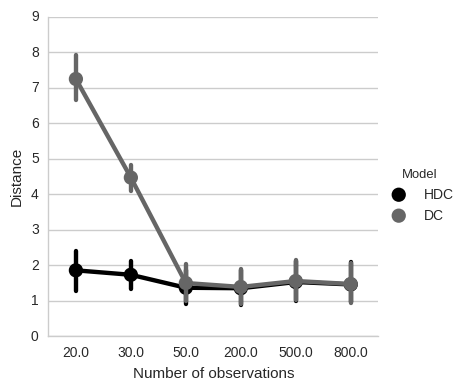
\includegraphics[width=\linewidth]{images/Eval-HDC-Bhattacharya-Distance.png}
    \caption{Bhattacharyya distance}
\end{subfigure}
\begin{subfigure}{.45\textwidth}
  \centering
  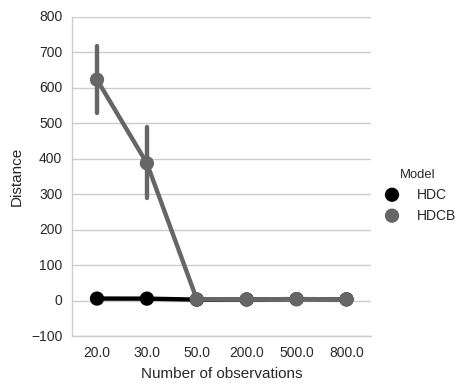
\includegraphics[width=\linewidth]{images/Eval-DC-KL-Distance.png}
    \caption{Kullback–Leibler divergence}
\end{subfigure}

\caption[DC, HDC Model Validation]{Measure of the distance between the learned probabilities and ground truth for models DC and HDB. The x-axis represents the different sample size.}
\label{fig:eval-B-KL-evaluation}
\end{figure}

Distances between the learned and the ground truth probabilities, learned using increasing number of observations is depicted in Figure~\ref{fig:eval-B-KL-evaluation}. The left plot is the Bhattacharyya distance while the right plot is the KL distance. We can observe that with increasing number of observations the distance is reduced. With around 50 observations both the models  completely converged with the ground truth.  

From the figure we can also conclude that when the observations are very few the HDC model performs better than the DC model. This validates that when some time periods which dont have enough observations the hyper prior added in hierarchical model shares information between time periods. HDC model performs better than DC model when the observations are few but as the observations increase there is no considerable difference in their learnings.

\section{Model Accuracy}

We have validated the working of the models on synthetic dataset in this section we validate HDC model on real world dataset. The aim of the experiments is to learn human location preference on real world dataset of location of a human in a house. We employ two methods for evaluating the performance of preference learning models. In addition to the traditional \emph{accuracy} measurements, we also evaluate the models based on the \emph{mean time to find the person}.  In the following section we explain the data collection procedure, data processing to information and then the two evaluation procedures.
 
\subsection{Aruba Dataset}
In our thesis, we have used a  publicly-available  dataset Aruba, published by the Lincoln Center for Autonomous Systems (LCAS). The dataset is of a person's location in a home collected at a smart apartment by the Center for Advanced Studies in Adaptive Systems (CASAS) \cite{aruba} .

The testbed where the dataset was collected is a  three-bedroom apartment located on the Washington State University that is part of CASAS smart home project \cite{aruba}. 


\begin{figure}
    \centering
    \begin{subfigure}[b]{0.4\textwidth}

        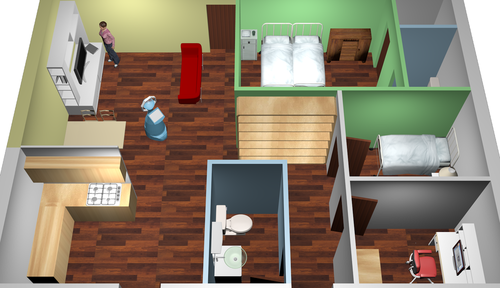
\includegraphics[width=\textwidth]{images/aruba-flat.png}
        \caption{Aruba apartment visualization}
        \label{aruba}
    \end{subfigure}
    ~ %add desired spacing between images, e. g. ~, \quad, \qquad, \hfill etc. 
      % (or a blank line to force the subfigure onto a new line)
    \begin{subfigure}[b]{0.5\textwidth}
        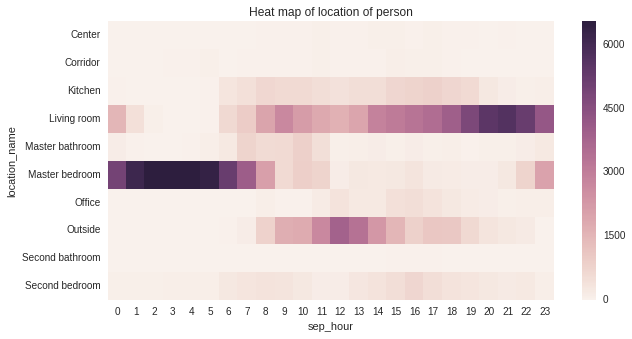
\includegraphics[width=\textwidth]{images/aruba-data.png}
        \caption{Heatmap}
        \label{fig:eval_gt}
    \end{subfigure}

    \caption[Aruba apartment visualization]{Aruba apartment visualization and Aruba dataset heatmap. In the heatmap, the x-axis are the locations of the home, y-axis are the hours of the day. The intensity of the color in each box indicates the number of times the person is present in that location. Higher the intensity means more time is spent by the person in that location at that time.}
    \label{aruba-visual}
\end{figure}

As shown in Figure~\ref{aruba}, the smart apartment test bed includes three bedrooms, one bathroom, a kitchen, and a living / dining room.  The apartment is equipped with motion sensors distributed approximately 1 meter apart throughout the space. The Aruba dataset was extracted from these motion sensor dataset provided by CASAS. The dataset contains the location of a person in the apartment every minute for 16 weeks.

We process the dataset and  order it as a  (hour,location) tuple. We visualize the dataset as a heatmap over locations distributed over different periods. As explained in chapter~\ref{sec:Problem formulation}, we try to learn daily patterns by dividing the observations into per hour periods. As we can see there are some prominent patterns present which can be learned. For example the usage of the bedroom, living room, outside and kitchen.

A histogram visualization of the observations over different location in the home is show in Figure~\ref{aruba-hist}

\begin{figure}[htp]
\centering
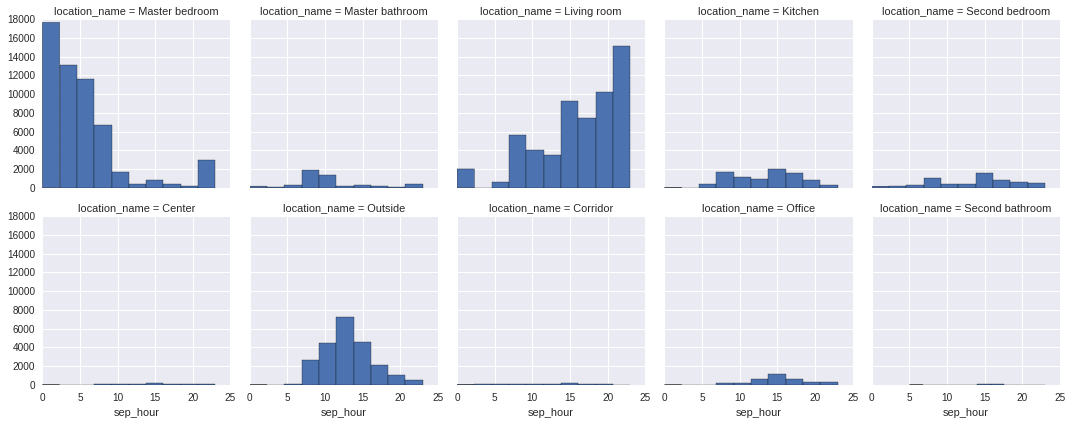
\includegraphics[width=\textwidth]{images/aruba-hist.png}
\caption[Aruba dataset histogram]{Aruba Dataset Histogram : Each box corresponds to histogram of each locations. The x - axis represents the time of the day (0-24) }
\label{aruba-hist}
\end{figure}


\subsection*{Sparsification}
Aruba dataset is a large dataset as compared to an person location dataset we assume the robot will be able to generate. The Aruba dataset has recordings of every minute for 118 days, which is 161280 readings.
On the contrary the assumed dataset which will be collected by the robot by autonomously roaming in a home will be just 3-5 readings per day.
So for simulating the sparsity in the object location dataset we will sparsify the ARUBA dataset by random selecting only selecting 3-5 readings each day.

After sparsification by randomly selecting 5 readings per day the dataset is reduced to 590 observations. The heatmap the of the sparsified dataset is shown in Figure~\ref{aruba-reduced-hist}. 

\begin{figure}[htp]
\centering
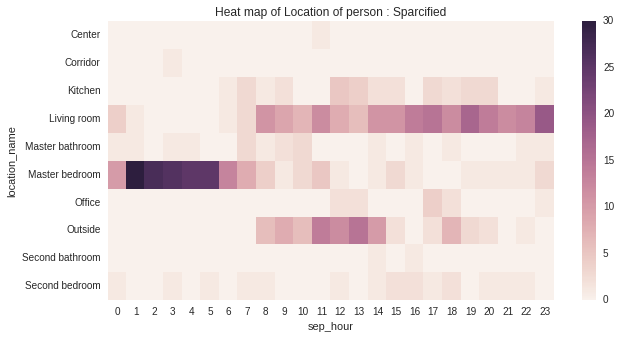
\includegraphics[width=\textwidth]{images/aruba-reduced-heatmap.png}
\caption[Aruba sparcified dataset heatmap]{Aruba sparcified dataset heatmap :The x-axis are the locations of the home, y-axis are the hours of the day. Compared to the complete observations the sparcified data set the patterns are not distinct}
\label{aruba-reduced-hist}
\end{figure}

\FloatBarrier


\subsection{Comparison With State-Of-Art Machine Learning Algorithms}

In this section we evaluate the predictive capabilities of our learned model. The accuracy of the predictions are measured and then compared with other state of the art machine learning algorithms. Two state-of the-art machine learning algorithms: Support Vector Machine (SVM)\cite{boser1992training, cortes1995support} and Random Forest \cite{breiman2001random, geurts2006extremely}. Scikit-learn \cite{sklearn_api} implementation of the algorithm were used for testing.

The goal of learning users location preference is to predict the location of the user based. We interpret the problem as a supervised machine learning with known input and outputs.In supervised learning the data comes a finite learning set $L =  (X, y)$ where, $X = input values$ and $y = output values$. 
For our problem statement the input is single feature, the time of the observation $X = [time]$, the output is the location of the person $y=[location]$

The learning was conducted using training set of different sizes, ranging from 0.0003\% (484 observations i.e. around 5 observations per day by the robot) to 0.2\% (32256 observations) of the dataset. The remaining data was used as testing set. The accuracy score for the classification is plotted in Figure~\ref{fig:SVM_vs_DCM}. 

\begin{figure}
    \centering
    \begin{subfigure}[b]{0.44\textwidth}
        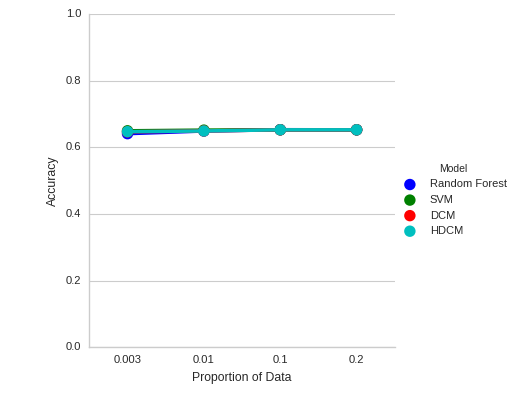
\includegraphics[width=\textwidth]{images/svm_vs_HDCM.png}
    \end{subfigure}
    \begin{subfigure}[b]{0.44\textwidth}
        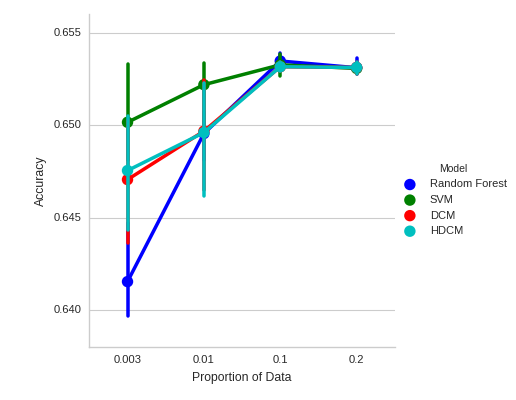
\includegraphics[width=\textwidth]{images/svm_vs_HDCM_zoomed.png}       
    \end{subfigure}
    
    \caption[Comparison with SVM and Random Forest]{ Comparison with SVM and Random Forest. The right plot is the zoomed view between 0.64 to 0.65}
    \label{fig:SVM_vs_DCM}
\end{figure}

As per the accuracy plot there is no considerable difference between the accuracy of  SVM, Random Forest, DC and HDC . Also the maximum accuracy is around 0.64\% , which doesn’t increase even with increasing number of observations. 


\subsection{Search time evaluation}
The models were also evaluated on the basis of the \emph{search time} to find the person. As mentioned above the goal of modelling human presence is to predict the persons location and reduce the time of search. Thus by calculating the time required to search the person based on the predictions of the model we can evaluate the accuracy of the learning.

\cite{krajnik_wheres_2015} in their seminal paper have proposed a path-planning search algorithm. This algorithm is used to determine the shortest path to be taken by the robot based on each locations probability. Thus it goes first to the most probable location first, then to other locations in decreasing order of the probabilities. \cite{krajnik_wheres_2015} solve the problem of learning preference of user location using temporal models. Two temporal models, frequency map enhancement  model  (FreMEn) and periodic Gaussian model (PerGaM) were used to learn the location preferences. 

We compare our developed model HDC along-with the FreMEn model based on the search time. A 'Static' model represented by static probability is used as a reference. Out of the 16 weeks of the Aruba dataset, first 4 weeks were used by \cite{krajnik_wheres_2015} to learn the models and last 12 weeks were used for testing. While in our case we learned using the sparse Aruba dataset  (~550 observations), and testing using same the last 12 weeks as above.

\begin{figure}[htp]
\centering
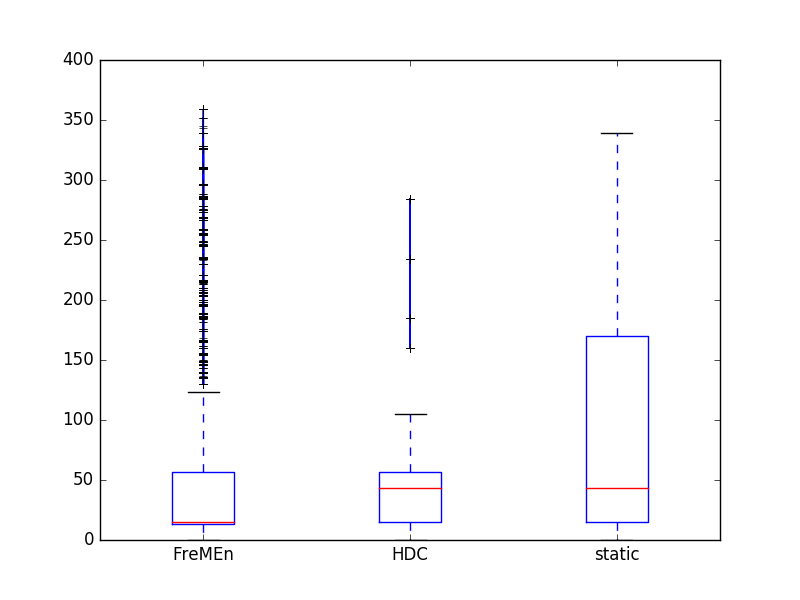
\includegraphics[width=\textwidth]{images/box_plot_fremen_hdc.png}
\caption[Search time evaluation]{Search times for different models}
\label{fig:search_time}
\end{figure}

As shown in Figure~\ref{fig:search_time} that compared to the stationary models the temporal model and our Bayesian models perform better in search time. The average search time of the temporal models are better than the Bayesian model.

\section{Discussions}

In this chapter, we presented probabilistic model to learn user location preferences.  In chapter \ref{chapter:occupancy} the models captured knowledge about each location separately, while in this chapter the models are able to capture knowledge about multiple locations in a single model. 

In an extensive experiments on synthetic dataset, we found that our model is capable of learning underlying patterns in user preferences. In first set of experiments we did a sanity check of our learning by visualizing the learned probability. Then we compared DC and HDC model and validated that addition of a hyper-prior improves learning when the observations are sparse. Furthermore, we evaluated the performance of the models predicting capability on a real world dataset, where the predictive accuracy results were around 63\% . The reason for such low accuracy result even with increasing number of dataset, can be explained by \cite{Bishop20120222} reasoning of ``Large" dataset. The author explains that learning is bad in some computationally large  (size) dataset as their statistical size in relation to the model is small. For example, consider a dataset with single input variable and single output variable with linear relationship. In such a dataset the model can learn with modest (20) examples even in the presence of noise. Such a dataset is computationally small but statistically large. However, a image dataset with millions of images for doing object detection is computationally large but statistically small, as it may contain only a tiny fraction of the different possible combinations. The Aruba dataset can be described as a computationally large but the statistically small dataset.

Finally, we compared the search time required by the robot to find the person in the home. The average search time of the model is reduced than the static search timings, but the median search time is very high as compared to the temporal model, FreMEn \citep{krajnik_wheres_2015}. One of the reasons can be that our models had a hour level dataset while FreMEn was learned at minute level dataset. Thus by learning user preferences the robot can make informed decisions that decrease the search time.
% section   (end)







%######################################################################

\chapter{Knowledge-enabled fault tolerant object search}
\label{cha}

Efficient searching for objects in the environment is one of the application for the knowledge being learned from object locations. The learned knowledge is as heuristics to improve the search time of objects. There are 2 basic methods in which we can use the learned knowledge as heuristics, first we can search for objects in the decreasing order of the learned probabilities or alternatively we can use the descriptive model to predict based on its learned probabilities. However the probabilistic representation of the learned knowledge can be used in ingenious way to solve more complex problems. Markov Decision Process (MDP) based planners can use the learned probabilities in their decision process to make more informed decisions. To illustrate this flexibility we have used the learned probabilities to make a sequential decision search algorithm which can accommodate the recognition failure in the vision algorithms.
\missingfigure{Image with false detection}
Household robots need to be able to recognize the objects they’re supposed to search and manipulate. But while object recognition is one of the most widely studied topics in artificial intelligence, even the best object detectors still fail much of the time. As a result there are very much possibilities that even though the search algorithm has provided the correct location the object detector might fail to locate the object. An alternative will be provide a search algorithm which can accommodate the object detector failures. All these object detectors along with the detection also publish the confidence(probability) of the detection. The proposed algorithm here combines both the \emph{detection probability} and the \emph{learned probability} of the objects and provide sequential decisions for the next location to search.

\section{Search as a decision Framework}
\todo[inline, caption={search1}]{Introduce the topic name}
\todo[inline, caption={search2}]{Add the 2 papers as the related work of probabilistic search in robotics}
\todo[inline, caption={search3}]{ and that the below model is a reduced version and simplified model}

The  contributions  of  this  paper  include  the  formulation of the search control problem as a decision-making problem rather  than  a  sensing  task,  where  measures  associated  with decisions,  e.g.  confidence  and  robustness  of  the  decision or  time  until  the  decision  is  made,  are  used  to  design  an appropriate  control  policy.  Our  formulation  of  the  search problem  as  a  detection  problem  also  allows  us  to  include practical  sensor  artifacts  (such  as  false  alarms  and  missed detections)  which  have  not  be  completely  considered  in other  formulations  [6]  of  the  search  problem.


A Decision-Making Framework for Control Strategies
in Probabilistic Search
Timothy H. Chung and Joel W. Burdick

A probabilistic framework for object
search with 6-DOF pose estimation 
\todo[inline]{robotics search in robots as POMDP in its related work}
\section{Model}
The idea is use the learned knowledge of the object locations as the first guess (prior ) of the probabilities that the object in question is located in each of the possible object locations. The prior probabilities suggest which location to search first. If the object is not found in that location, the prior probabilities are then updated (yielding the posterior), and the process is repeated until the object is found. 

Assume that the domain of interest is a home we call $D_s$, which is made up of n spatial areas. Let $Y_i = 1$ if the object is in the \emph{i}th location, and then $Y_i = 0$ if it is not; $ i = 1, .... , n$. Now as discussed above object detectors can fail to detect the object. So, let $Z_i = 1$ if the object is found in the \emph{i}th location, and $Z_i = 0$ if not.

We can define two terms \emph{detection probability},
\begin{equation}
	p_i = Pr(Z_i = 1| Y_i =1), \qquad  i = 1,...,n,
\end{equation}
which is a conditional probability, and the \emph{occurrence probability},
\begin{equation}
	\pi_i = Pr(Y_i = 1),\qquad  i = 1, .... , n.
\end{equation}

This can be expressed in probabilistic programming form:
\begin{gather}
	Z_i | Y_i \sim Bernoulli (Y_i, p_i), \qquad  i  = 1,....,n \\
	Y_i \sim Bernoulli(\pi_i),\qquad   i = 1,...,n,
\end{gather}

where, the occurrence probability {$\pi_i$} is given by the learned probabilities, while the detection probability {$\pi_i$} is provided by the object detector algorithm.

Now, assume that hte \emph{i}th location is searched by the robot and the object is not found (i.e., $Z_i = 0$). In that case, the probability that the object is in the \emph{i}th location is updated using Bayes' Theorem. This yields the posterior probability,

\begin{align*}
	Pr(Y_i = 1 | Z_i = 0) &= \frac{Pr(Z_i = 0|Y_i=1)Pr(Y_i=1)} {Pr(Z_i=0)} \\
	                       &= \frac{Pr(Z_i = 0| Y_i =1 )Pr(Y_i =1)}{Pr(Z_i=0|Y_i =1)Pr(Y_i = 1) + Pr(Z_i=0|Y_i=0)Pr(Y_i=0)} \\
	                       &= \frac{(1 - p_i)\pi_i}{(1 - p_i)\pi_i + (1)(1 - \pi_i)} \\
	                       &= \frac{(1 - p_i)\pi_i}{1 - p_i\pi_i}
\end{align*}

where we assume that there are no false-positive detection (i.e., $Pr(Z_i =0| Y_i = 0) = 1$). Note that the new posterior is less than the prior probability $\pi_i$ as the object was not observed.

Since the object is not found in the searched location, then this should also affect the posterior probability in the other grid boxes. For example, consider the \emph{j}th location, where $j \neq i$. Then,
\begin{align*}
	Pr(Y_j = 1 | Z_i=0) &= \frac{Pr(Z_i = 0 | Y_j = 1)Pr(Y_j = 1)}{Pr(Z_i = 0)} \\
	                    &= \frac{\pi_j}{ 1 - p_i\pi_i}
\end{align*}

Thus, the posterior probability of the object being the \emph{j}th location is greater than the prior probability $\pi_j$ . These new posteriors will then become the next prior probabilities is a sequential procedure that would determine the next location to search.

\section{Example}
\todo{split as 2 example , 1 with high detection probablity 0.9 and other with 0.6}
\todo{show the different sequence}
Suppose we have a domestic robot which has learned the location probabilities of a cup in a home. The robot has learned that the cup can be found 3 locations in the home, thus the domain for search can be defined as $D_s = \{cupboard, table, dishwasher \}$ . 
Now lets assume the robot has been in the room for long enough and made some observations. Based on these observations it learns the occurrence probabilities as $p_i = \{ 0.8, 0.1, 0.1\}$ . The object detector for the cup has a \emph{detection probability} of $p_{cup} =  0.6$ .

As you can see there is a strong probability of finding the cup in the cupboard. The algorithm selects to search the cupboard. But the object detector fails and is not able to detect the cup. If we are not using the algorithm the robot will move on to the next location to search the cup in the next location.


\missingfigure{Illustration of the proabbiliities and how they change with each observation}

However our algorithm on the failure detection will update its probabilities and the updated posterior probability will be $ p_i = \{ 0.44, 0.27, 0.27\}$ and it still selects to search the cupboard for the next time. This illustrates the algorithm understands the limitation in the object detector and updates its beliefs to accommodate this limitation and make better \emph{informed} decisions.  

 
\section{Evaluation}
hey you didnt think about evaluation ? 
% chapter  (end)

\chapter{Cleaning robot scenario}

If you grew up watching the Jetsons, the idea of having a robot helper that cleans and cooks for your family has always been a fantasy. People want to have a robot do the housework and the good news is that great minds are working on it.

Elon Musk announced back in June that his OpenAI robotic institute was working on developing software that would enable off-the-shelf robots to do household chores and various other engineers are working on robots that could accomplish cleaning and organizing tasks.

 In order for a robot to clean an entire house, it would have to be able to fully understand its environment and make decisions based on the state of each room -- something that is beyond the current abilities of artificial intelligence. 
 \cite{http://www.treehugger.com/gadgets/want-robot-clean-your-house-youll-have-wait-bit-longer.html}
 
\chapter{Modeling}
Data Modeling.
Each data scientist in practice uses tools and viewpoints from
both
of
Leo Breiman's modeling cultures:

Generative modeling
, in which one proposes a stochastic model that could have generated
the data, and derives methods to infer properties of the underlying generative mechanism.
This roughly speaking coincides with traditional Academic statistics and its o shoots.
31

Predictive modeling
, in which one constructs methods which predict well over some some
given data universe { i.e.  some very speci c concrete dataset.  This roughly coincides with
modern Machine Learning, and its industrial o shoots.

\chapter{Useful wordings}

\begin{itemize}
	\item Experience based machine intelligence \textbf{and the benefits it could engender such as} fixing model-specific problems and product efficiency \textbf{are good reasons to enable network connectivity}.
	\item Not all data is created equal, and certainly not all of it is meaningful to collect and display.
\end{itemize}

%\listoftodos
\end{document}
